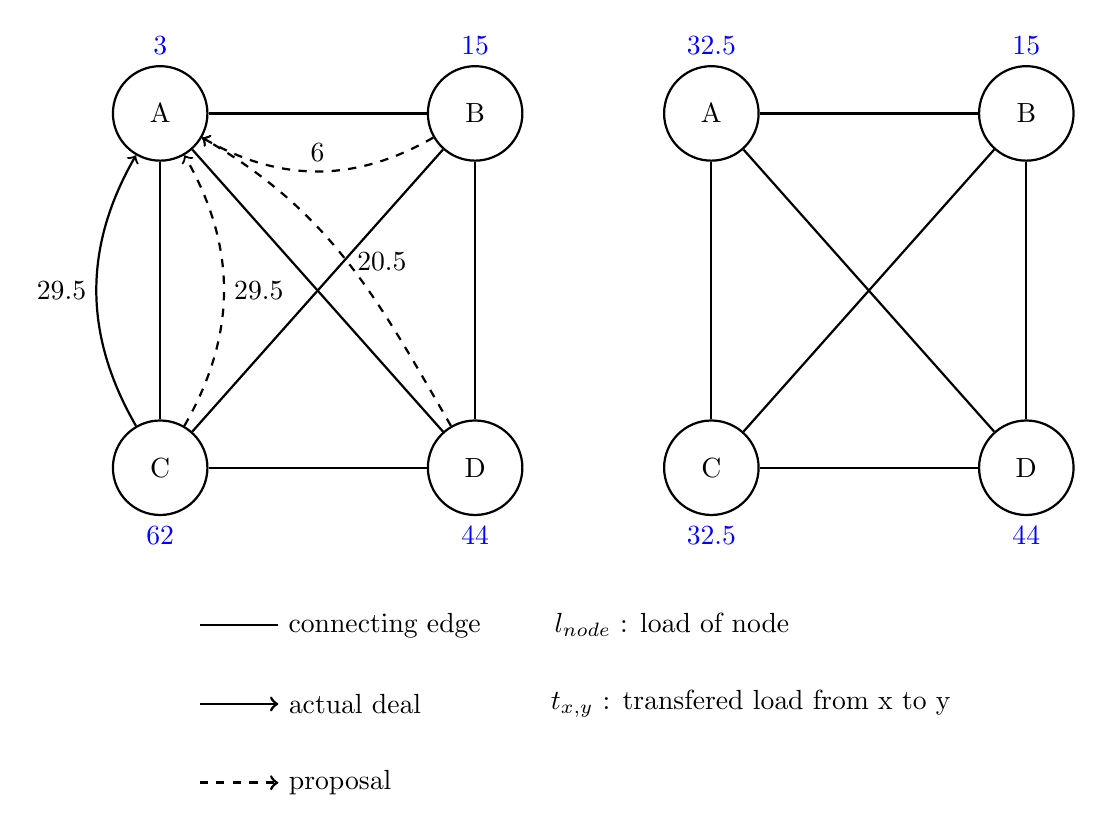
\begin{tikzpicture}[ thick, main node/.style={circle, draw, minimum size=1.2cm}]

    % First graph
    \node[main node] (A1) at (0.5,4.5) {A};
    \node[main node] (B1) at (4.5,4.5) {B};
    \node[main node] (C1) at (0.5,0) {C};
    \node[main node] (D1) at (4.5,0) {D};
    
    \node[above, color=blue] at (A1.north) {3};
    \node[above, color=blue] at (B1.north) {15};
    \node[below, color=blue] at (C1.south) {62};
    \node[below, color=blue] at (D1.south) {44};
    
    \draw (A1) -- (B1);
    \draw (A1) -- (C1);
    \draw (A1) -- (D1);
    \draw (B1) -- (C1);
    \draw (B1) -- (D1);
    \draw (C1) -- (D1);

    % Second graph
    \node[main node] (A2) at (7.5,4.5) {A};
    \node[main node] (B2) at (11.5,4.5) {B};
    \node[main node] (C2) at (7.5,0) {C};
    \node[main node] (D2) at (11.5,0) {D};
    
    \node[above, color=blue] at (A2.north) {32.5};
    \node[above, color=blue] at (B2.north) {15};
    \node[below, color=blue] at (C2.south) {32.5};
    \node[below, color=blue] at (D2.south) {44};
    
    \draw (A2) -- (B2);
    \draw (A2) -- (C2);
    \draw (A2) -- (D2);
    \draw (B2) -- (C2);
    \draw (B2) -- (D2);
    \draw (C2) -- (D2);

    \draw[->] (C1) to[out=120, in=240] node[left] {$29.5$} (A1);
    \draw[dashed, ->] (C1) to[out=60, in=300] node[right] {$29.5$} (A1);
    \draw[dashed, ->] (B1) to[out=210, in=330] node[above] {$6$} (A1);
    \draw[dashed, ->] (D1) to[out=120, in=330] node[right] {$20.5$} (A1);

    % Legend in the middle below the graphs
    \begin{scope}[shift={(3,-2)}]
        % Horizontal line
        \draw (-2,0) -- (-1,0) node[right] {connecting edge};
        % Long right arrow
        \draw[->, line width=1pt] (-2,-1) -- (-1,-1) node[right] {actual deal};
        % Long right dashed arrow
        \draw[->, dashed, line width=1pt] (-2,-2) -- (-1,-2) node[right] {proposal};
        
        % Load notation
        \node at (4,0) {$l_{node}$ : load of node};
        \node at (5,-1) {$t_{x,y}$ : transfered load from x to y};
    \end{scope}

\end{tikzpicture}